\subsection{Afgrænsning af løsningsfelt}
For at visualisere hvilken afgrænsning af løsningsfeltet, der nu er foretaget, har vi, ud fra ovenstående problemanalyse, fremstillet figur \ref{fig:p1_skitser}, der viser løsningsfeltet for det initierende problem. Figuren viser på den lodrette akse hvem der styrer visualiseringen af lamper, og den vandrette akse viser, hvor lamperne visualiseres. I feltet er fire løsningsmuligheder vist.

\begin{figure}[H]
  
  \centering
  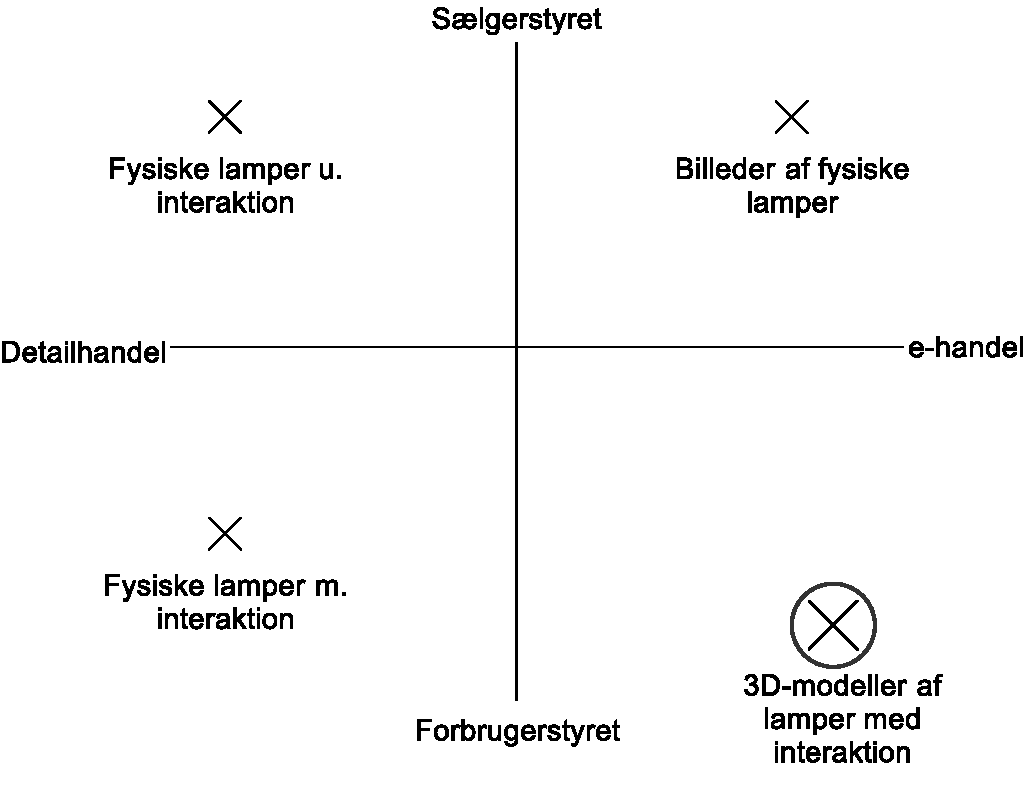
\includegraphics[width=10cm]{p1_skitser}
  \caption{Illustrerer lønningsfeltet til initierende problem, hvor det afgrænsede løsningsfelt er markeret med en cirkel.}
  \label{fig:p1_skitser}
\end{figure}

Herunder er de fire løsningsmuligheder, vist på figur \ref{fig:p1_skitser}, beskrevet:
\begin{enumerate}
  \item fysiske lamper uden interaktion, som er de lamper lampebutikker udstiller i fysiske butikker, men som forbrugeren ikke har mulighed for interaktion med, det vil sige at dette ofte er lamper som er slukket.

  \item fysiske lamper med interaktion, som er de lamper lampebutikker udstiller i fysiske butikker og som brugeren bl.a.\ kan slukke og tænde for, altså have interaktion med.

  \item billeder af fysiske lamper på e-butikker. Her har kunden mulighed for at se et billede af lampen, men kun fra de vinkler og i den kontekst som lampebutikken har valgt.

  \item 3D-modeller af fysiske lamper m.\ interaktion på e-bukker. Her har kunden mulighed for at se et 3D billede af lampen samt rotere lampen, og herved se hvordan lampens belysning er fra de ønskede vinkler, og ikke kun i den kontekst som lampebutikken vælger det. 
\end{enumerate}

Figuren viser nu at det er løsningsmulighed 4, som der afgrænset til i løbet af problemanalysen, og vi dermed har fravalgt løsningsmulighed 1-3 på baggrund af problemanalysen. Dette gør at der nu kan opstilles en endelig problemformulering, som ligger op til en løsningsmulighed 4.